In this section, we will address the different existing solutions to compute the fractional part division.
% \footnote{explicit base 2 notation}
\begin{equation}
\frac{(1.f_1)}{(1.f_2)}
\end{equation}

When implemented in hardware, different non-negligible trade-offs come into play.

There are three main families of division algorithms \cite{muller_hardware_2010}. 

\begin{itemize}

\item Digit-recurrence (DR) algorithms, such as the family of SRT algorithms named after Sweeney, Robertson, and Tocher, %[344, 408]
generalize the paper-and-pencil algorithm. They produce one digit of the result at each iteration. Each iteration performs three tasks (just like the pencil-and-paper method): (i) determine the next quotient digit, (ii) multiply it by the divider, and (iii) subtract it from the current partial remainder to obtain a partial remainder for the next iteration.
In binary, there are only two choices of quotient digits, 0 or 1; therefore, the iteration reduces to one subtraction, one test, and one shift. 
A binary digit-recurrence algorithm can therefore be implemented on any processor as soon as it is able to perform integer addition.

One important thing about digit-recurrence algorithms is that they are exact. Starting from fixed-point numbers $X$ and $D$, they compute at iteration $i$ an $i$-digit quotient $Q_i$ and a remainder $R_i$ such that the identity $X = DQ_i + R_i$ holds.
For floating-point purposes, this means that all the information needed for rounding the result is held in the pair $(R_i, Q_i)$. In practice we limit the number of digits for the division result to $p$, introducing an approximation.
%In practice, to round to precision $p$, one needs $p$ iterations to compute $Q_p$, then possibly a final addition on $Q_p$ depending on a test on $R_p$.


\item Polynomial approximation can also be used to evaluate $1/x$ to the required accuracy. %[430].
Note that, mathematically speaking, functional iterations evaluate a polynomial in the initial approximation error. % [88].

\item Functional iteration algorithms generalize the Newton-Raphson iteration for approximating the function $1/x$. They make sense mostly on processors having a hardware multiplier. The number of iterations is much less than in digit-recurrence algorithms ($\mathcal{O}(\log p)$ versus $\mathcal{O}(p)$), but each iteration involves multiplications and is, therefore, more expensive. These latter two methods may be combined.
\end{itemize}

\subsection{Approximated reciprocal}

In order to compute an approximated reciprocate, we can think of exploiting the Taylor series technique\footnote{Wikipedia. 2022. "Taylor series." Wikimedia Foundation. Last modified October 4, 2022. https://en.wikipedia.org/wiki/Taylor\_series.} around $ 0.75 = mean([0.5, 1))$.


However, this approach presents some inconveniences:
\begin{itemize}
\item it requires $6$ fixed-point products\footnote{$3$ due to 3rd-order term $x*x*x*3.1604\dots$ + $2$ + $1$},
\item it is accurate just around the point where the series is expanded, as shown in figure \ref{fig:relative_error_00001}.
\end{itemize}
A way to circumvent the latter issue comes from employing the Chebyshev polynomials. They are used to provide the best approximation not only around a given point but across an interval.
As a trade-off, the better control over the accuracy across this interval comes at the cost of increased computational complexity, compared to the plain Taylor expansion.


Applying the third-order Chebyshev polynomials \cite{Hale2015}formula to $1/x$ across the interval $(0.5, 1)$ we obtain
\begin{equation}\label{equ:3rd_order_Chebyshev_polynomial_equation}
f_{cp_3} = 5.65685 - 11.75737x + 10.64818x^2 - 3.54939 x^3 + \mathcal{O}(x^4)
\end{equation}
which, from the visual comparison with other approximations (figure \ref{fig:relative_error_00001}) seems to return a better approximation of the $1/x$ function across the interval. However, similarly to the Taylor expansion, it still suffers from the long chain of fixed-point products.

A different idea comes from \cite{drom}, with a fast technique for approximated reciprocate computation. In particular, this approach offers three main advantages: (i) no dividers, except division by powers of $2$; (ii) minimal amount of multipliers; (iii) integer arithmetic only.


The following routine is indeed hardware friendly, as it employs just two integer multiplications and a bit shift.

\begin{verbatim}
def reciprocal(a):
    b = 1.466 - a
    c = a * b
    d = 1.0012 - c
    e = d * b
    out = e * 4
    return out
\end{verbatim}


\begin{figure}
    \centering
    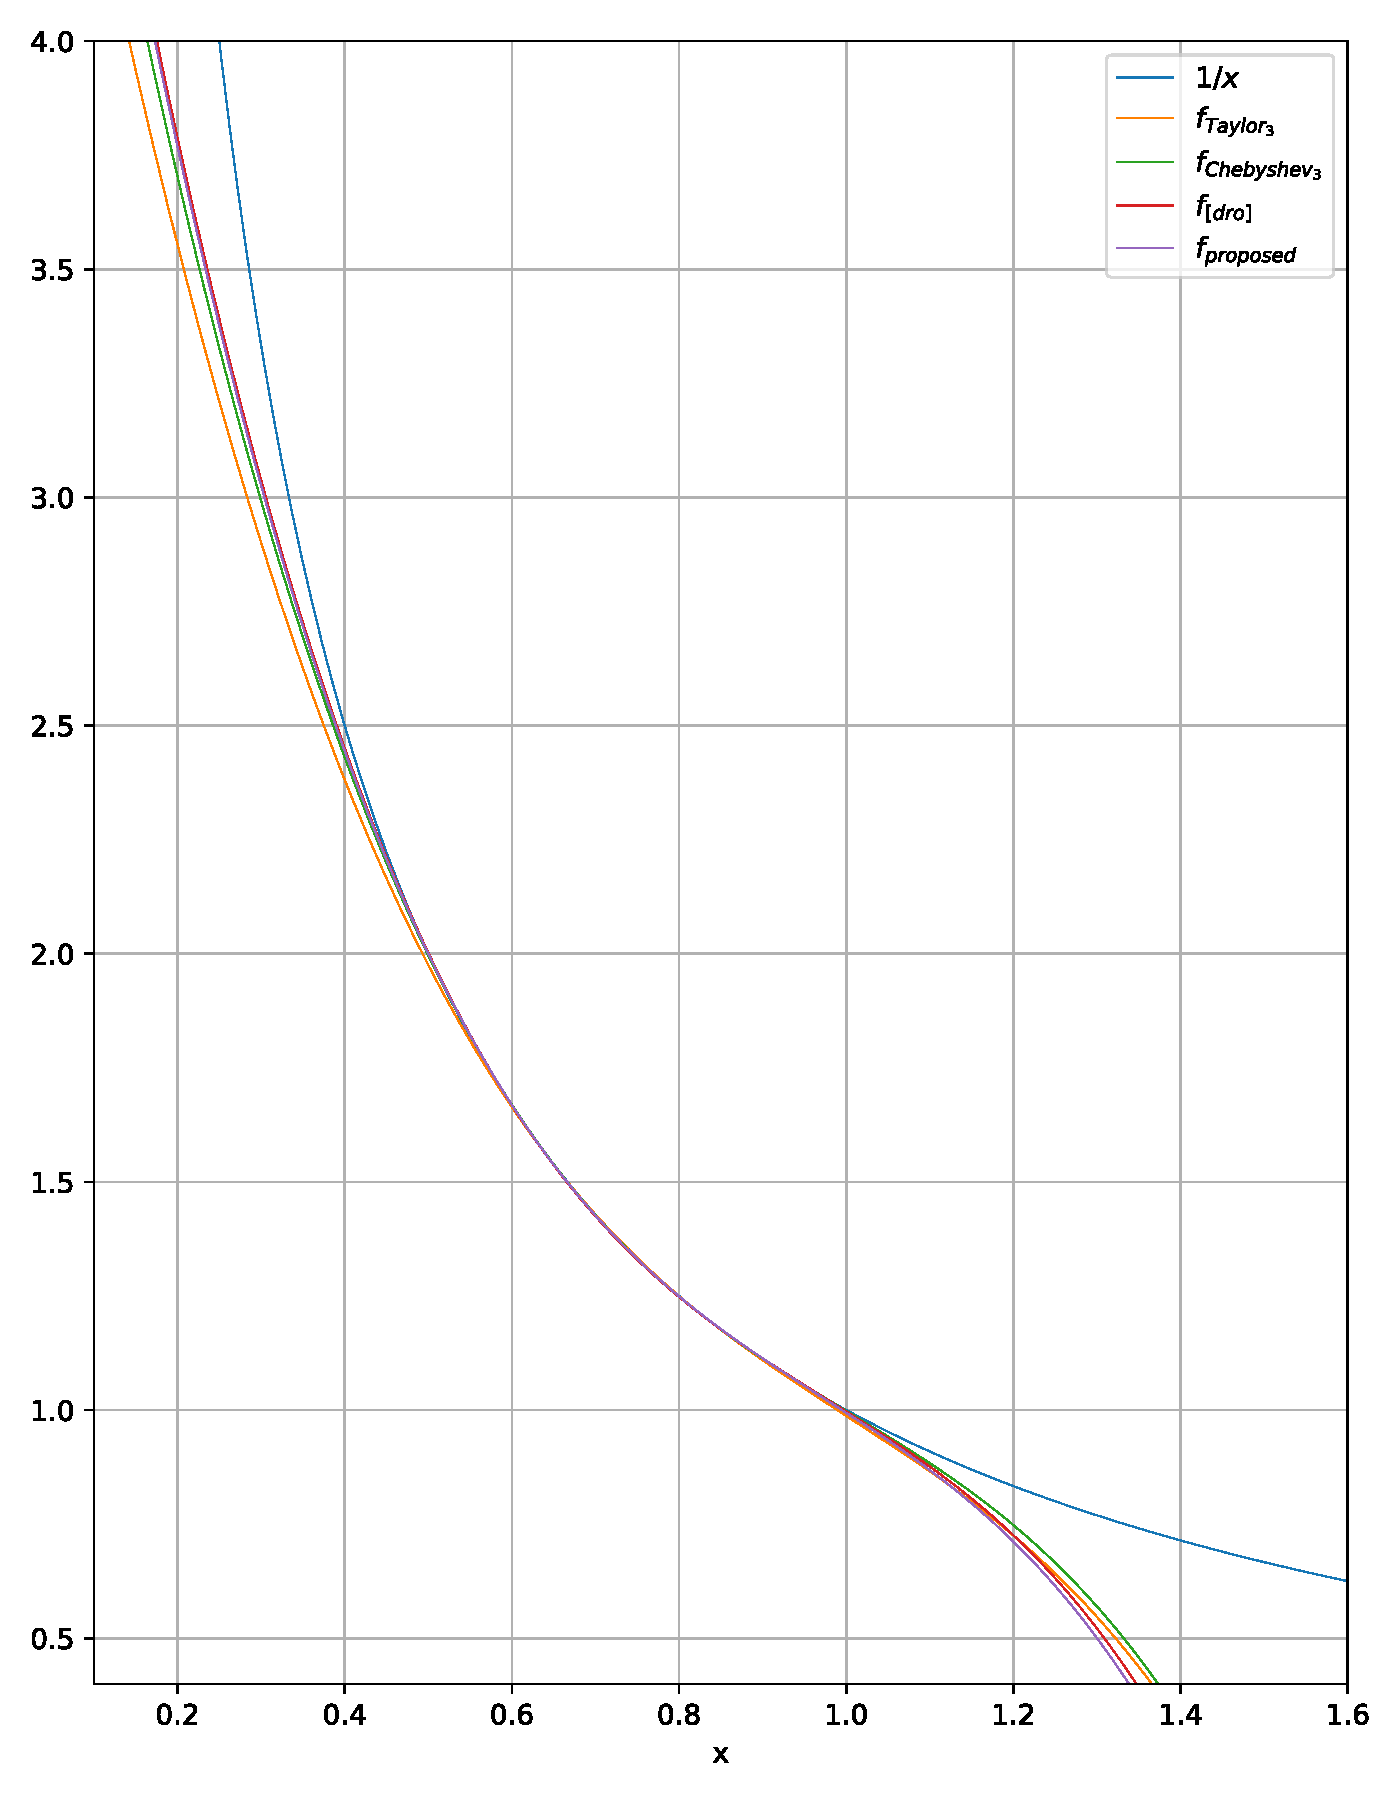
\includegraphics[width=0.75\textwidth]{figures/reciprocate_real_vs_taylor_vs_drom.pdf}
    \caption{Comparison of $1/x$ vs \cite{drom} vs 3rd order Taylor polynomial vs 3rd order Chebyshev polynomial vs proposed solution (i.e. optimized \cite{drom})}
    \label{fig:0203012875432985734}
\end{figure}

\begin{figure}
    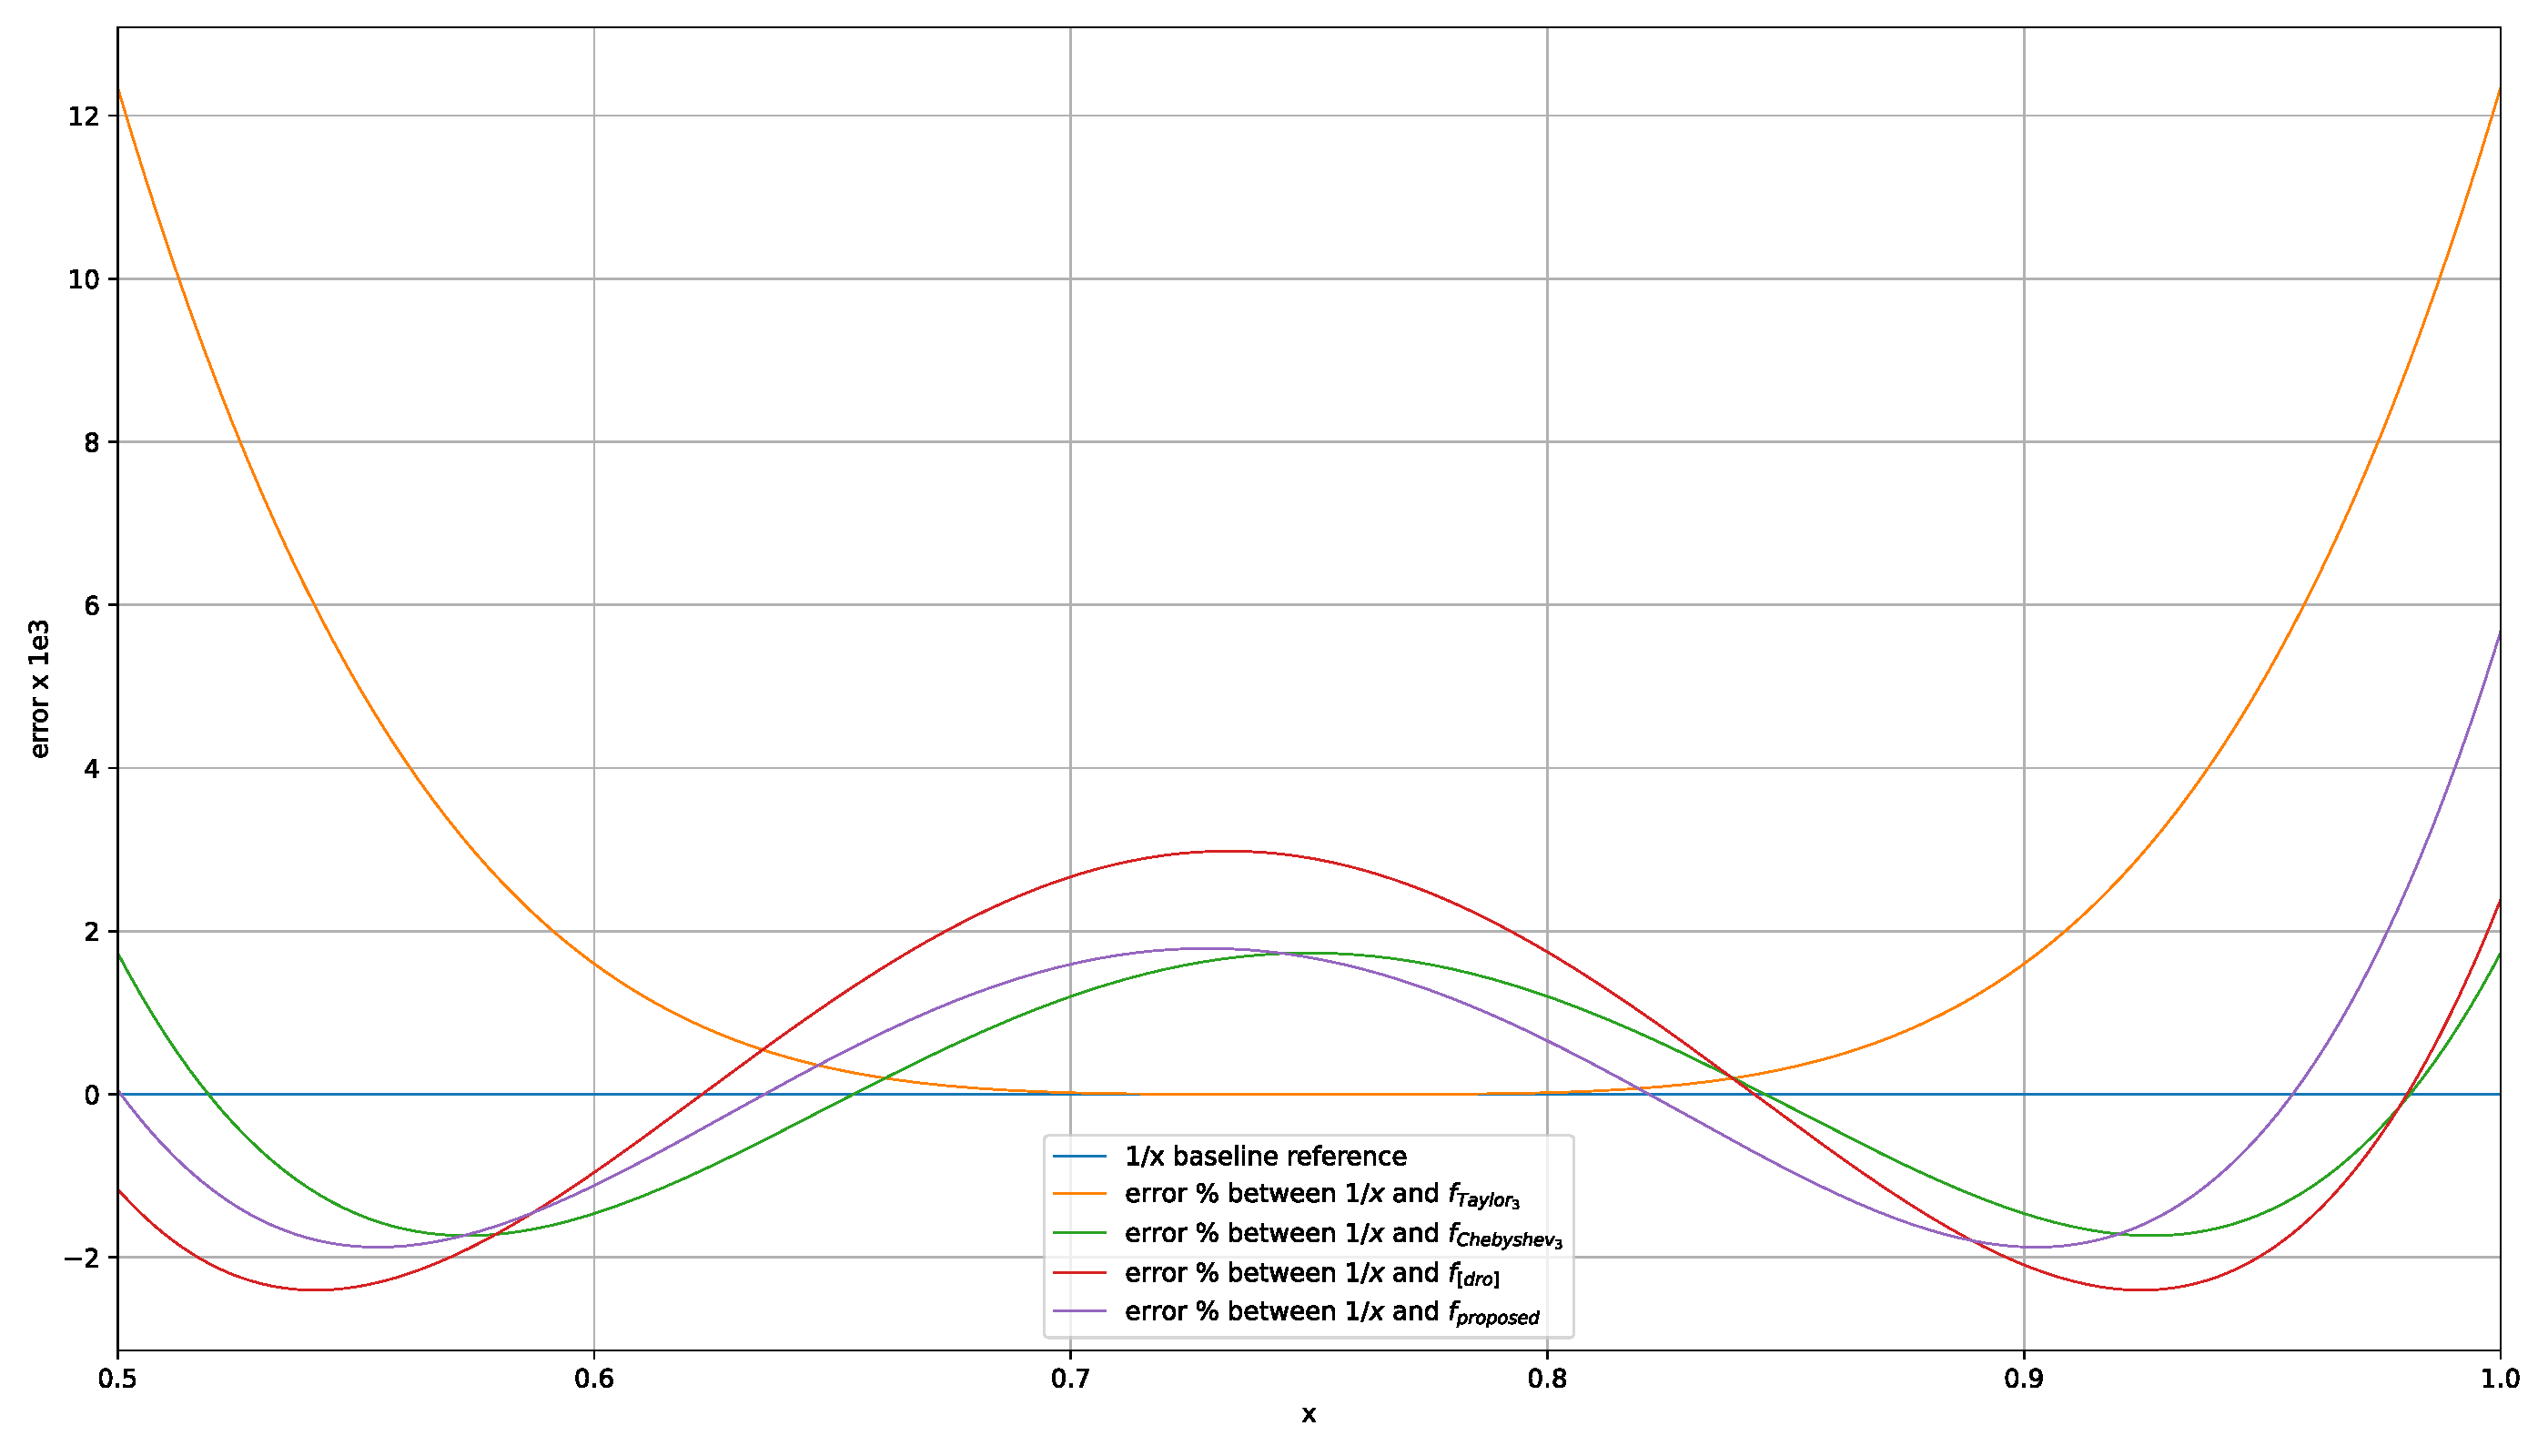
\includegraphics[width=1\textwidth]{figures/reciprocate_real_vs_taylor_vs_drom_error.pdf}\caption{Relative error against reference $1/x$}\label{fig:relative_error_00001}
\end{figure}
\begin{figure}
    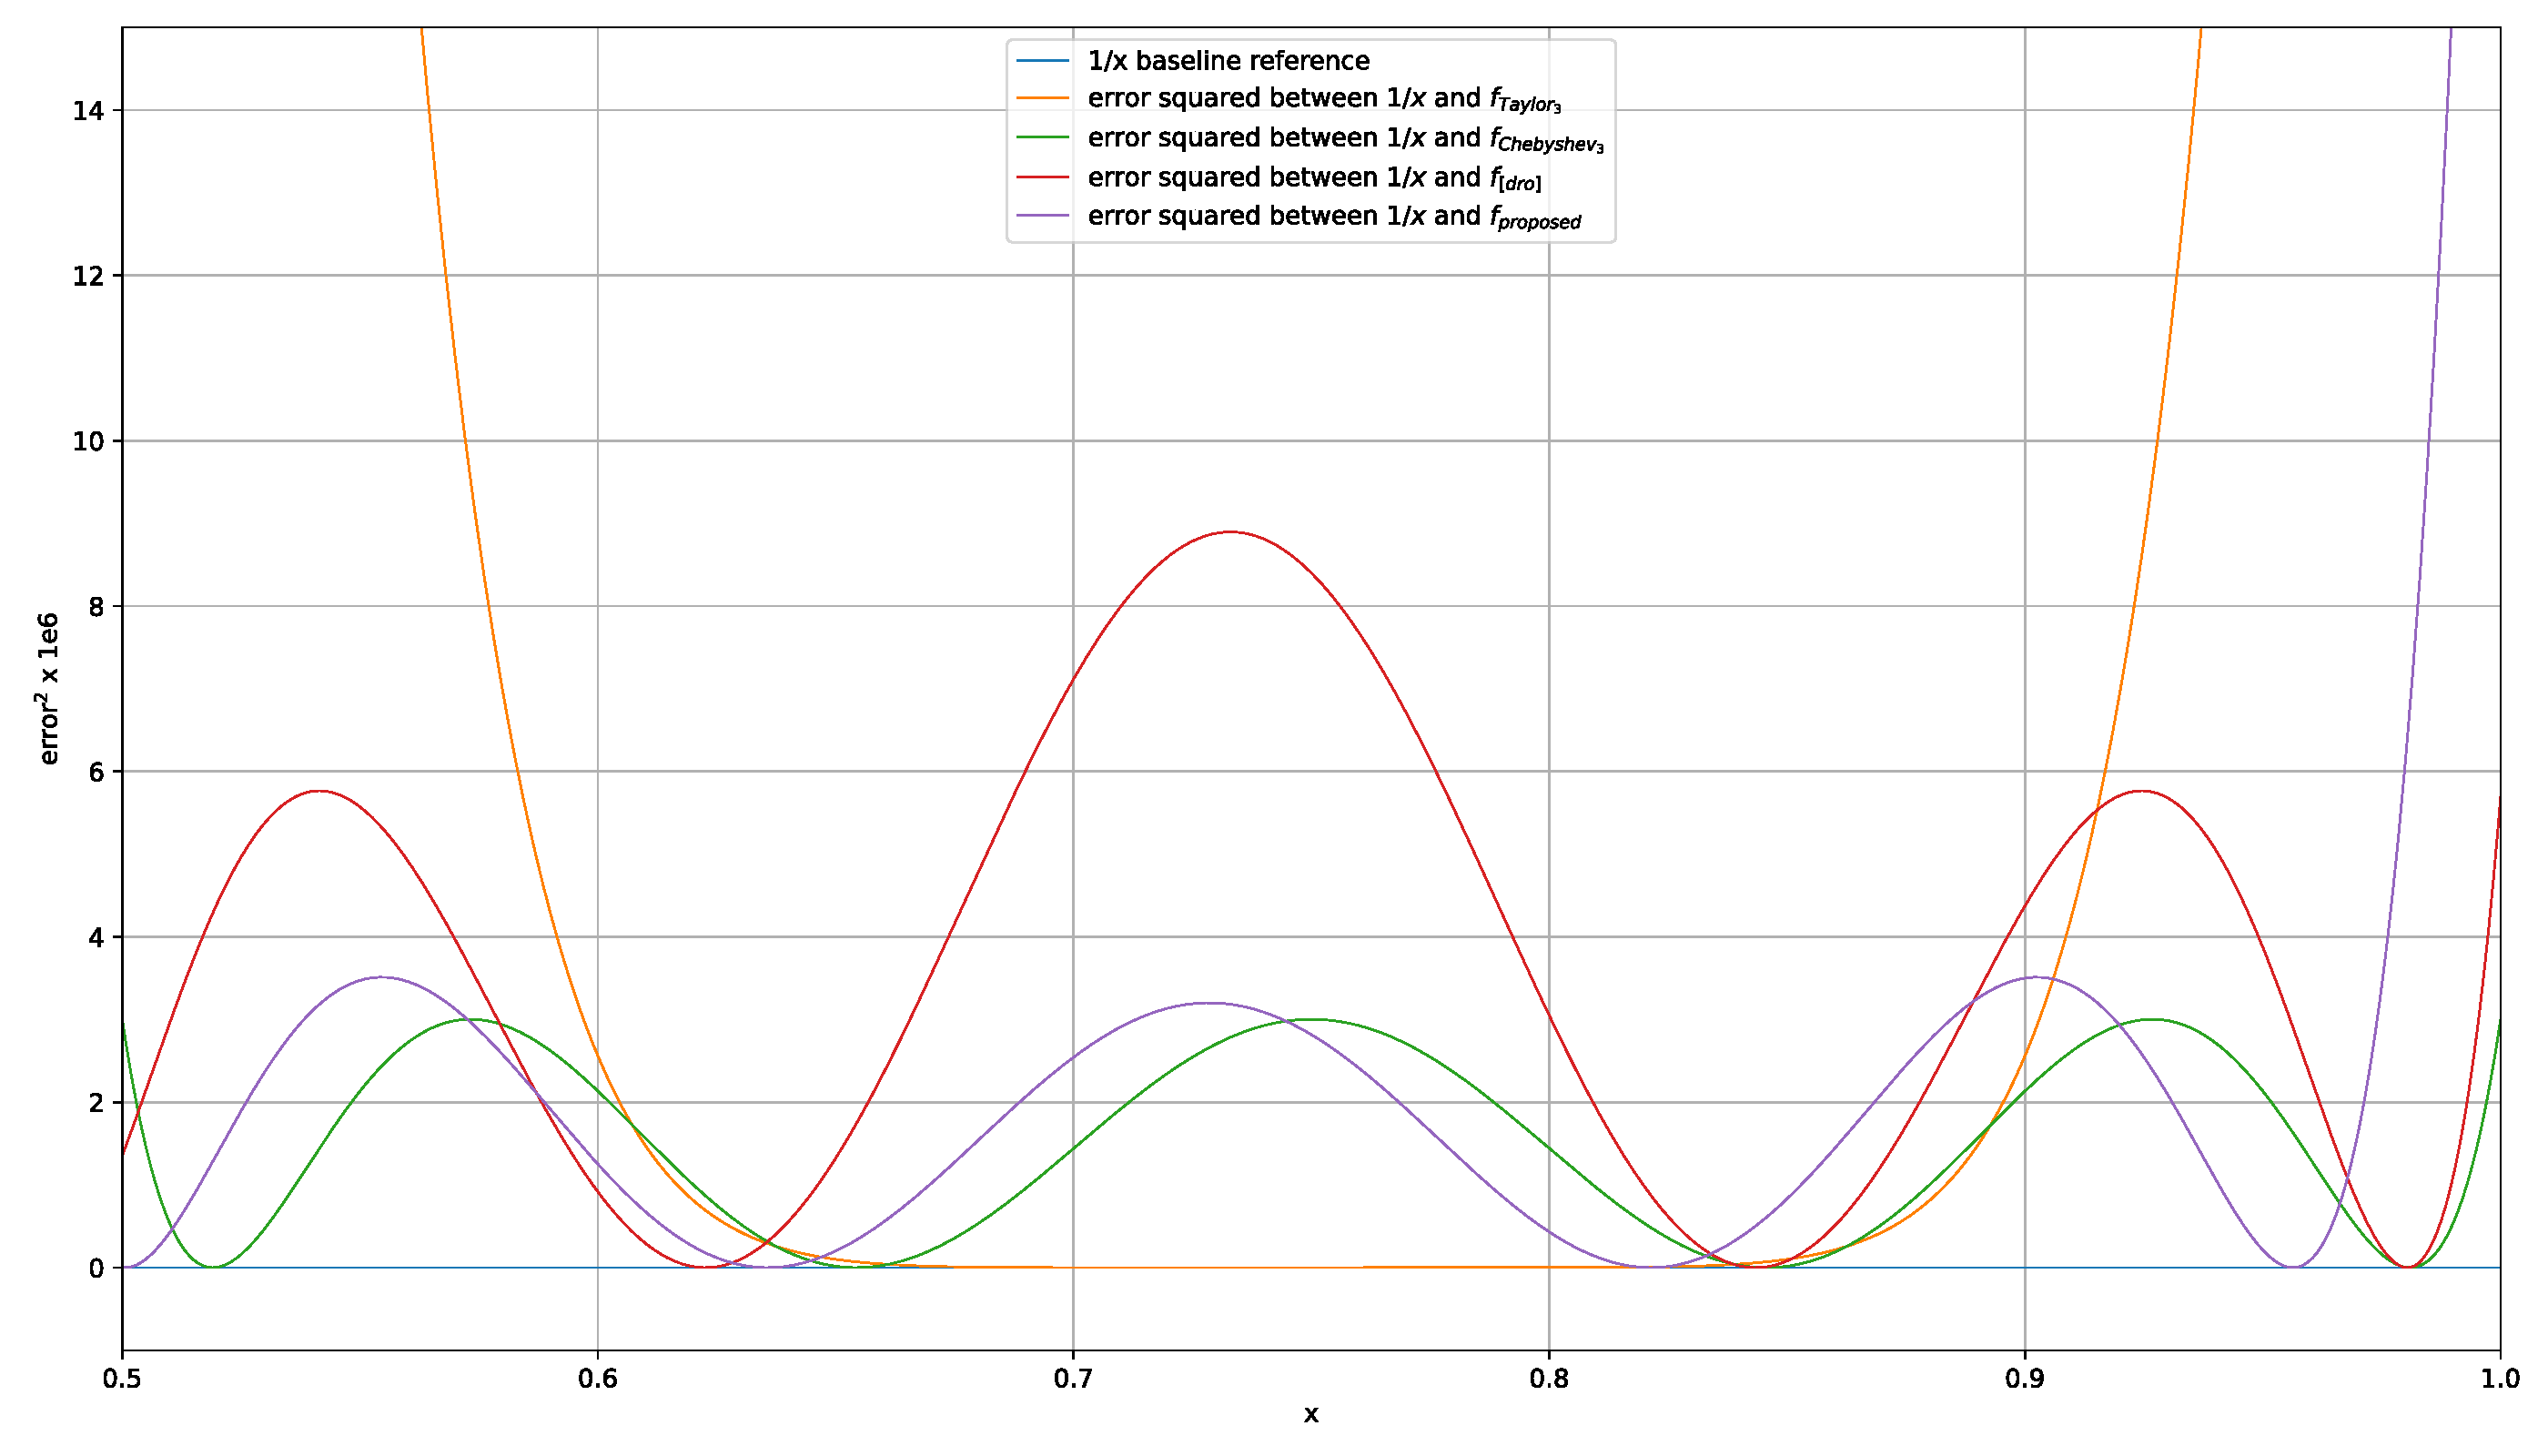
\includegraphics[width=1\textwidth]{figures/reciprocate_real_vs_taylor_vs_drom_error_squared.pdf} 
    \caption{Squared relative error against reference $1/x$}
    \label{fig:020301280980435232835} 
\end{figure} 

If we expand the routine into a  third-order polynomial (\ref{equ:expanded_drom_modified_polynomial}, \ref{equ:expanded_drom_0000}) similar to the previous ones, we can see that this is a modified Chebyshev polynomial with the highest grade coefficient rounded to the closest power of two -- $4$ in this case.
This constraint on the highest grade coefficient reduces the long-chained multiplication required by the original Chebyshev polynomial approximation (\ref{equ:3rd_order_Chebyshev_polynomial_equation}), with a slight degradation in accuracy.
\begin{equation}\label{equ:expanded_drom_modified_polynomial}
\begin{aligned}
f(a, k_1, k_2) &= 4 \cdot e = 4 \cdot d \cdot b = \\
&= 4 \cdot (k_2 - c) \cdot (k_1 - a) = \\
&= 4 \cdot (k_2 - a \cdot b) \cdot (k_1 - a) = \\
&= 4 \cdot [k_2 - a \cdot (k_1 - a)] \cdot (k_1 - a) = \\
&= 4 \cdot (k_2 - k_1 a + a^2) \cdot (k_1 - a) = \\
&= 4 \cdot (k_1 k_2 - k_2 a - k_1^2 a + 2 k_1 a^2 - a^3) = \\
&= 4 k_1 k_2 - 4(k_1^2 + k_2) a + 8 k_1 a^2 - 4 a^3
\end{aligned}
\end{equation}

Let $e^2$ be an error function to compare the accuracy of the different methods presented before. The function $e^2$ corresponds to the underlying area below the curves in Figure \ref{fig:020301280980435232835}. The value $rerr$ indicates the relative error between the real and the approximated function\footnote{$|rerr|$ would have given a comparably meaningful Function of Merit, however, the function must be differentiable in the entire domain, hence $rerr^2$}.


\begin{figure}
    \centering
    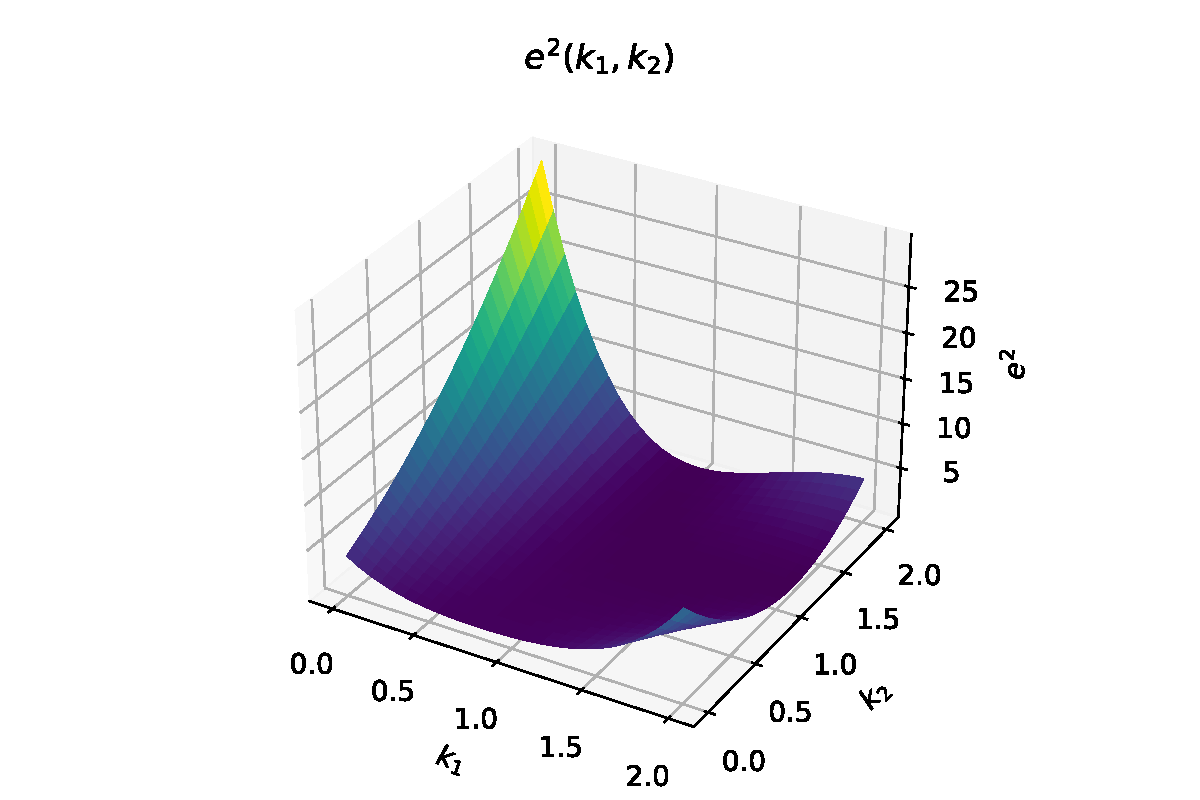
\includegraphics[
        %scale=1
        width=1\linewidth,]{figures/3d_plot_error_squared.pdf}
    \caption{\\$e^2(k_1, k_2)$}
    \label{fig:errorsquared3dplot}
\end{figure}
    
Let $f_{[dro]}$ be the Chebyshev polynomial defined using the coefficients as in \cite{drom}:

\begin{equation}\label{equ:expanded_drom_0000}
\begin{aligned}
f_{[dro]}(a) &= f(a, k_1=1.466, k_2=1.0012) = \\
&= 5.8710368 - 12.601424 a + 11.728 a^2 - 4 a^3
\end{aligned}
\end{equation}

 \begin{equation}\label{equ:equation_e_squared_k1k2}
            \begin{aligned}
            e^2(k_1, k_2) &=  \int_{1/2}^{1} rerr^2(x, k_1, k_2)\ dx = \\
            &= \int_{1/2}^{1} \left( \frac{f(x, k_1, k_2) - 1/x}{1/x} \right)^2 dx = \\
            &= \int_{1/2}^{1} \left( \frac{k_1 k_2 - 4(k_1^2 + k_2) x + 8 k_1 x^2 - 4 x^3 - 1/x}{1/x} \right)^2 dx = \\
            &= \frac{31 k_{1}^{4}}{10} - \frac{15 k_{1}^{3} k_{2}}{2} - \frac{21 k_{1}^{3}}{2} + \frac{14 k_{1}^{2} k_{2}^{2}}{3} + \frac{93 k_{1}^{2} k_{2}}{5} + \\ 
            &+ \frac{1339 k_{1}^{2}}{84} - \frac{15 k_{1} k_{2}^{2}}{2} - \frac{75 k_{1} k_{2}}{4} - \frac{375 k_{1}}{32} + \frac{31 k_{2}^{2}}{10} + \\ 
            &+ \frac{577 k_{2}}{84} + \frac{5507}{1440}
            \end{aligned}
        \end{equation}
        
We may want to know which are the optimal $k_1$ and $k_2$ such that:
\begin{equation}\label{equ:opt_k1_k2_eq}
(k_{1_{opt}}, k_{2_{opt}}): \min\{e^2(k_1, k_2)\}
\end{equation} 

For that the following system of equations (\ref{equ:opt_k1_k2_eq}) must be solved:
\begin{equation}\label{equ:opt_k1_k2_eq_partial}
\begin{cases}
\dfrac{\partial}{\partial k_1} e^2(k_1, k_2) = 0 \\
\dfrac{\partial}{\partial k_2} e^2(k_1, k_2) = 0
\end{cases}
\end{equation} 
\iffalse
$$
\begin{cases}
k_{1_{opt}} = 1.4567844114901045 \\
k_{2_{opt}} = 1.0009290026616422
\end{cases}
$$
\fi
which gives $(k_{1_{opt}} = 1.4567844114901045,\ k_{2_{opt}} = 1.0009290026616422)$, yielding a $36.4\%$ improvement over \cite{drom}'s $e^2$. Figure \ref{fig:are_barplot} shows a comparison of the relative accuracy of the above-mentioned functions and techniques compared to $1/x$.

\begin{figure}
    \begin{center}
    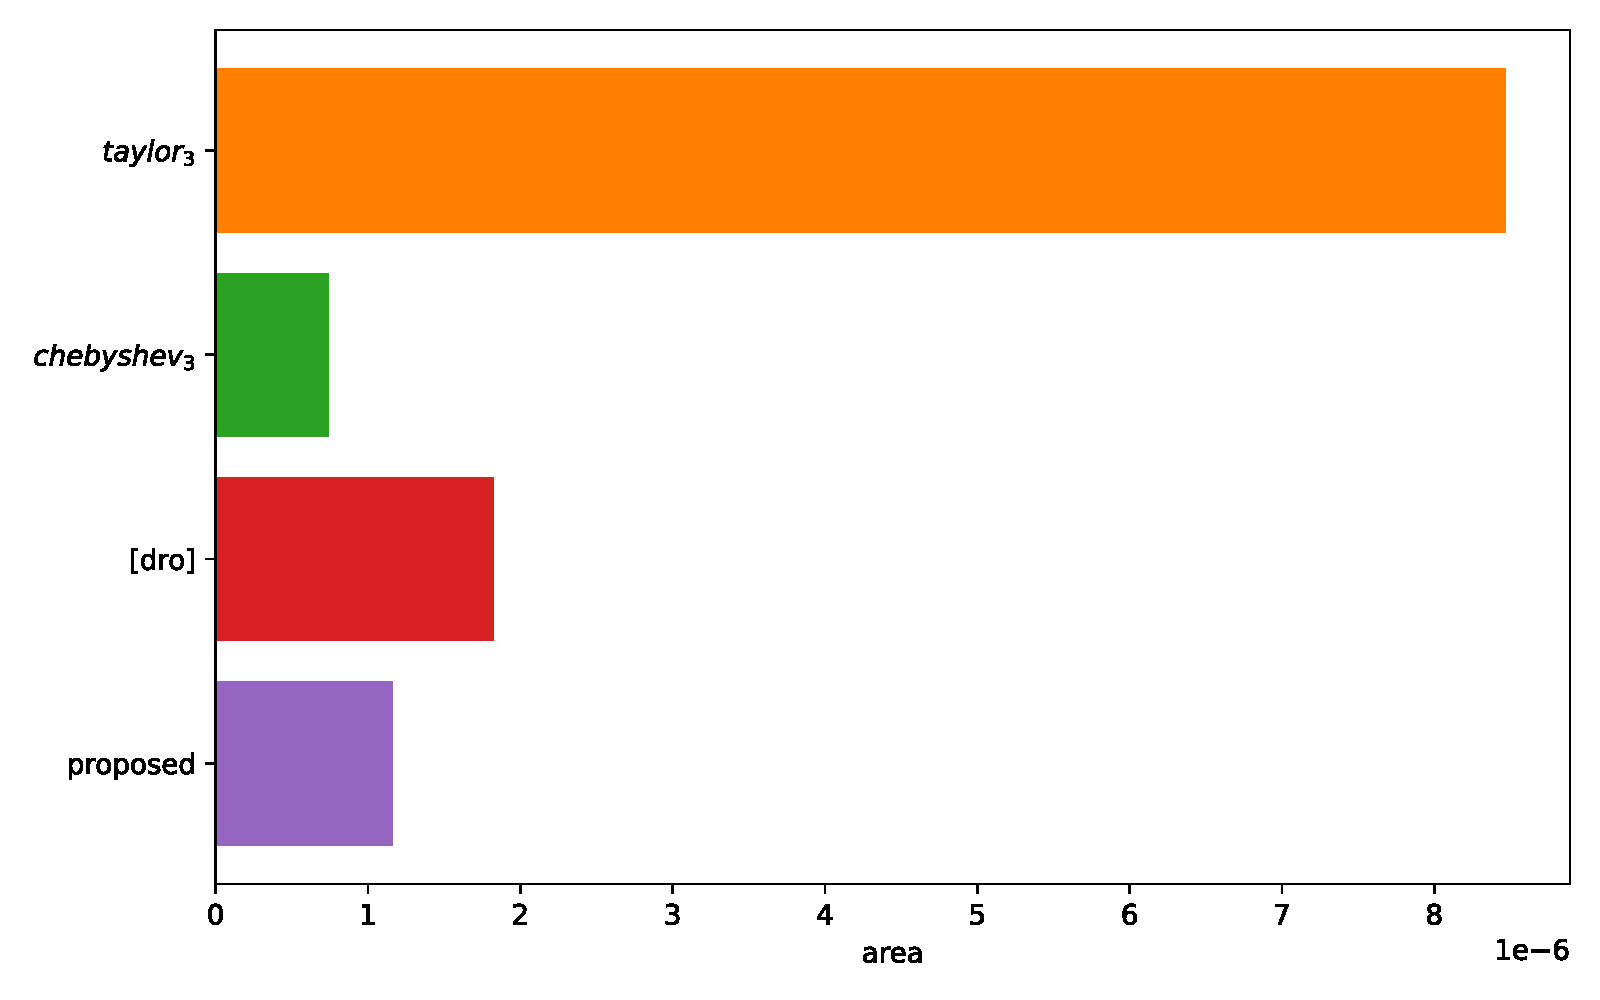
\includegraphics[width=0.4\textwidth]{figures/barplot_area_error.pdf}
    \caption{Barplot error area. $taylor_3$ vs $chebyshev_3$ vs \cite{drom} vs proposed}
    \label{fig:are_barplot}
    \end{center}
\end{figure}


Using the optimal $k_1$ and $k_2$ coefficients -- i.e. (i) Chebyshev-like polynomial, and (ii) highest grade coefficient being a power of $2$\footnote{so that the bit shift trick can be performed, as opposed to yet another multiplication} -- we can now use the following algorithm to perform the approximated reciprocal:

\begin{lstlisting}[label=alg:reciprocal_approx_modified_drom]
def reciprocal(a):
    b = k1_opt - a
    c = a * b
    d = k2_opt - c
    e = d * b
    out = e << 2
    return out
\end{lstlisting}

The numerical bounds of the result of each step in the algorithm can be determined so that we can set the correct fixed-point representation, allocating enough bits.

The input is a mantissa, hence contained in $[1, 2)$: in order to fit in the range required by the algorithm, that is $[0.5, 1)$, we divide by $2$, or, we just operate a one-bit right shift. Similarly, a division by $2$ is required when the algorithm terminates to restore the pre-normalization value.


Figure \ref{fig:reciprocal_unsigned_workflow} shows the flow of the procedure. 



\begin{itemize}
    \item \texttt{a} $\in [0.5, 1) \equiv A $ \dotfill \texttt{Fx<0, F>}
    \item \texttt{b} $\in (0.45702824, 0.95702824] $ \dotfill \texttt{Fx<0, F>}
    \item \texttt{c} $\in (0.45702824, 0.5307166278550605) $ \dotfill \texttt{Fx<0, 2F>}
    \item \texttt{d} $\in (0.47022002214493963, 0.54390841) $ \dotfill \texttt{Fx<0, 2F>}
    \item \texttt{e} $\in (0.24858150334349846, 0.4999731144222473) $ \dotfill \texttt{Fx<0, 3F>}
    \item \texttt{out} $\in (0.9943260133739938, 1.9998924576889892) $ \dotfill \texttt{Fx<1, 3F>}
\end{itemize}



    

\begin{figure}
    \centering
    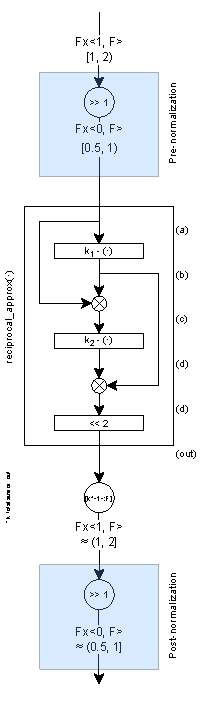
\includegraphics[width=0.28\textwidth]{figures/reciprocal_unsigned.drawio.pdf}
    \caption{Reciprocal unsigned workflow}
    \label{fig:reciprocal_unsigned_workflow}
\end{figure}

\subsection{Ahead-of-time reciprocal}\label{aot_reciprocal_lut_technique}

The previous solution presents a reduced result's precision (due to the approximated reciprocate) with the benefit of a reduction in required hardware resources.
Another solution called \textit{Ahead Of Time} computation of the reciprocate, helps with the accuracy drop seen before: the core idea is that instead of computing the reciprocate on-demand, we store the reciprocates inside a look-up table (as in \cite{PACoGen}). Such a look-up table takes $N$ bits representing the $N$ most significant bits of the fraction as input and will output the $M$ most significant bits of the reciprocate of the input.

\begin{figure}[h!]
    \begin{center}
    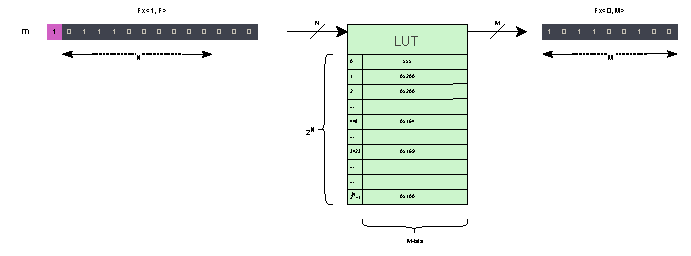
\includegraphics[width=1\textwidth]{figures/lut.drawio.pdf}
    \caption{Look Up Table example, taking P$\langle 16,1 \rangle(0x71c0)$'s mantissa as input}
    \label{fig:lut_drawio_example}
    \end{center}
\end{figure}

Concerning the same posit, $P\langle 16,1 \rangle(0x71c0)$, figure \ref{fig:lut_drawio_example} gives an example of the mechanism: i) the fraction field is adjusted to $N$ bits (this can be either a bit-expansion or a bit-compression); ii) the value represented by those bits is used to index the element in the look-up table resulting in the $M$ most significant bits of the reciprocate of the full input mantissa.

The lookup table gives another degree of freedom: $N$ and $M$ can be set independently from the posit size to account for the trade-off between resource utilization and required accuracy for the reciprocate.


\subsection{Newton-Raphson}\label{Newton_Raphson}


In numerical analysis, the Newton–Raphson method \cite{Hale2015_a} is a root-finding algorithm which produces successively better approximations of the roots of a real-valued function. The most basic version starts with a single-variable function $f$ defined for a real variable $x$, the function's derivative $f'$, and an initial guess $x_0$ for a root of $f$.
If the function satisfies sufficient assumptions and the initial guess is close, then the algorithm is guaranteed to converge to a root of $f$. The iterative scheme for the algorithm is shown in \eqref{equ:newon_raphson_generalized_equation}:

\begin{equation}\label{equ:newon_raphson_generalized_equation}
x_{n+1} = x_n - \frac{f(x_n)}{f'(x_n)}
\end{equation}

This technique can be exploited to solve the problem of interest by noticing that if we consider a function whose root is such that $x = 1/k$, e.g.
\begin{equation}
f(x) = \frac{1}{x} - k
\end{equation}
with derivative
$$
f'(x) = -\frac{1}{x^2}
$$
where $n$ is the number whose reciprocate we are after and $x$ the reciprocate itself, the Newton Raphson method gives
\begin{equation}
\begin{aligned}
x_{n+1} &= x_n - \frac{f(x_n)}{f'(x_n)} = \\
& = x_n - \frac{\dfrac{1}{x_n} - k}{-\dfrac{1}{x_n^2}} = \\
& = x_n\ (2 - k \cdot x_n)
\end{aligned}
\end{equation}
which yields a valid approximation so long as the initial guess $x_0 \in (0, 2/k)$, to not make the iteration diverge.


